\documentclass[11pt,letterpaper,onecolumn,notitlepage]{article}
\usepackage[english]{babel}
\usepackage[compact]{titlesec}
\usepackage[titles]{tocloft}
\usepackage{%
  float,
  amssymb,
  amsmath,
  graphicx,
  fullpage,
  textcomp,
  gensymb,
  hyperref,
  listings,
  caption,
  sectsty,
  bm,
  times,
  parskip,
  empheq
}
\usepackage[framed,numbered,autolinebreaks,useliterate]{../sty/mcode}

\lstset{breakatwhitespace=false}

\newcommand{\figurepath}{../fig/hw3}
\newcommand{\codepath}{../include/code/hw3}

\sectionfont{\fontsize{16pt}{16pt}\selectfont\bfseries\sffamily}
\subsectionfont{\fontsize{13pt}{13pt}\selectfont\sffamily}
\subsubsectionfont{\fontsize{12pt}{12pt}\selectfont\sffamily}
\paragraphfont{\fontsize{11pt}{11pt}\selectfont\bfseries}

\makeatletter
\renewcommand\section{\@startsection{section}{1}{\z@}%
{-3.5ex\@plus-1ex\@minus-0.2ex}%
{1.0ex\@plus0.2ex}%
{\fontsize{12pt}{12pt}\selectfont\bfseries\sffamily}}
\makeatother

\makeatletter
\renewcommand\subsection{\@startsection{subsection}{1}{\z@}%
{-3.5ex\@plus-1ex\@minus-0.2ex}%
{0.5ex\@plus0.2ex}%
{\fontsize{10pt}{10pt}\selectfont\bfseries\sffamily}}
\makeatother

%------------------------------------------------------------------------
\setlength\cftparskip{-3pt}
\setlength\cftbeforesecskip{1pt}
\setlength\cftaftertoctitleskip{1pt}
\cftsetindents{figure}{0em}{1.5em}
\makeatletter
\renewcommand{\@dotsep}{4.5}
\renewcommand{\cftdotsep}{4.5}
\renewcommand{\cftsecdotsep}{4.5}
\renewcommand{\@tocrmarg}{4.55em}
\makeatother
\renewcommand\cftsecfont{\normalfont}
\renewcommand\cftsecpagefont{\normalfont}
\renewcommand{\cftsecleader}{\cftdotfill{\cftsecdotsep}}
%------------------------------------------------------------------------

\titleformat{\chapter}[display]{\huge\bf}{Lecture \thechapter}{0pt}{\Large}

\title{\textbf{Title}}
\author{Daniel Wiese \\ Department of Mechanical Engineering \\ Massachusetts Institute of Technology}
\date{\today}

\begin{document}

  \begin{titlepage}
    \begin{center}
      \rule{\linewidth}{0.01in} \\[0.25in]
      {\huge\bfseries 16.323 Optimal Control}\\[0.4cm]
      \rule{\linewidth}{0.01in} \\[0.25in]

      \textsc{\LARGE Problem Set 3}\\[0.15in]
      \large Due: Tuesday, April 1, 2014 \\[1.0in]
      
\includegraphics[width=1.5in]{../fig/mit-seal.pdf}\\[3.0in]

      % Author and instructor
      \begin{minipage}{0.4\textwidth}
        \begin{flushleft} \large
          \emph{Author:}\\
          Daniel \textsc{Wiese}
          \vfill
        \end{flushleft}
      \end{minipage}
      \begin{minipage}{0.4\textwidth}
        \begin{flushright} \large
          \emph{Instructor:} \\
          Prof.~Steven \textsc{Hall} \\
        \end{flushright}
      \end{minipage} \\
      \vfill
    \end{center}
  \end{titlepage}

  \clearpage
  \section{Calculus of Variations}

  Find the curve $x(t)$ that minimizes the functional

  \begin{equation*}
    J(x)=\int_{0}^{1}\biggr\{\frac{1}{2}\dot{x}^{2}(t)+3x(t)\dot{x}(t)+2x^{2}(t)+4x(t)\biggr\}dt
  \end{equation*}

  and passes through the points $x(0)=1$ and $x(1)=4$.

  \subsection*{Answer}

  The given functional which we are trying to minimize is in the form $J(x)=\int_{0}^{1}g(x(t),\dot{x}(t),t)dt$ where

  \begin{equation*}
  g(x(t),\dot{x}(t),t)=\frac{1}{2}\dot{x}^{2}(t)+3x(t)\dot{x}(t)+2x^{2}(t)+4x(t)
  \end{equation*}

  We apply the Euler-Lagrange equation $\frac{\partial{}g}{\partial{}x}-\frac{d}{dt}\frac{\partial{}g}{\partial\dot{x}}=0$.
  We first evaluate the derivatives which go into the Euler-Lagrange equation as

  \begin{align*}
  \frac{\partial{}g}{\partial{}x}&=3\dot{x}+4x+4 \\
  \frac{\partial{}g}{\partial\dot{x}}&=\dot{x}+3x
  \end{align*}

  Now define $f(x(t),\dot{x}(t),t)=\frac{\partial}{\partial\dot{x}}g(x(t),\dot{x}(t),t)$ and evaluate $\frac{d}{dt}f(x(t),\dot{x}(t),t)$ by applying chain rule as

  \begin{equation*}
    \frac{d}{dt}f(x(t),\dot{x}(t),t)=
    \frac{\partial{}f}{\partial{}x}\frac{\partial{}x}{\partial{}t}+
    \frac{\partial{}f}{\partial\dot{x}}\frac{\partial\dot{x}}{\partial{}t}+
    \frac{\partial{}f}{\partial{}t}
  \end{equation*}

  With our definition $f=\dot{x}+3x$ from before we have

  \begin{equation*}
    \frac{d}{dt}\frac{\partial{}g}{\partial\dot{x}}=3\dot{x}+\ddot{x}
  \end{equation*}

  Now putting the whole Euler-Lagrange equation together we have

  \begin{equation*}
    3\dot{x}+4x+4-3\dot{x}+\ddot{x}=0
  \end{equation*}

  which can be simplified to

  \begin{equation*}
    \ddot{x}-4x=4
  \end{equation*}

  This equation needs to be solved subject to the given initial conditions.
  First solve the homogeneous equation $\ddot{x}-4x=0$.
  Propose $x_{h}(t)=Ae^{Bt}$.
  Twice differentiating gives $\ddot{x}_{h}(t)=B^{2}Ae^{Bt}$.
  Plugging into the homogeneous equation we have $B^{2}-4=0\Rightarrow B=\pm2$.
  This gives $x_{h}(t)=A_{1}e^{2t}+A_{2}e^{-2t}$.
  The particular solution is a constant $x_{p}(t)=-1$.
  The total solution then is

  \begin{equation*}
    x(t)=-1+A_{1}e^{2t}+A_{2}e^{-2t}
  \end{equation*}

  Now we need to solve for the constants $A_{1}$ and $A_{2}$ using the boundary conditions.

  \begin{align*}
    x(0)&=-1+A_{1}+A_{2}=1 \\
    x(1)&=-1+A_{1}e^{2}+A_{2}e^{-2}=4
  \end{align*}

  From the first equation we have $A_{1}=2-A_{2}$.
  Plugging this into the second equation we get

  \begin{align*}
    2e^{2}-A_{2}e^{2}+A_{2}e^{-2}&=5
    \Rightarrow \\
    A_{2}(e^{-2}-e^{2})=5-2e^{2}
  \end{align*}

  And so we can solve for $A_{2}$ and then $A_{1}$, and plug those into the solution.

  \begin{empheq}[box=\fbox]{alignat=3}
    x(t)&=-1+A_{1}e^{2t}+A_{2}e^{-2t} \\[6pt]
    A_{1}&=2-\frac{5-2e^{2}}{e^{-2}-e^{2}} \\[6pt] % chktex 8
    A_{2}&=\frac{5-2e^{2}}{e^{-2}-e^{2}} % chktex 8
  \end{empheq}

  \clearpage
  \section{Variational Approach to Optimal Control}

  Find the control that transfers the following system,

  \begin{align*}
    \dot{x}_{1}(t)&=x_{2}(t) \\
    \dot{x}_{2}(t)&=-x_{2}(t)+u(t)
  \end{align*}

  from $x_{1}(0)=0$, $x_{2}(0)=0$ to the line $x_{1}(t)+5x_{2}(t)=15$, and minimizes

  \begin{equation*}
    J=\frac{1}{2}(x_{1}(t_{f})-5)^{2}+\frac{1}{2}(x_{2}(t_{f})-2)^{2}+\frac{1}{2}\int_{t_{0}}^{t_{f}}u^{2}dt
  \end{equation*}

  Solve for the state and cost ate equations analytically.

  \subsection*{Answer}

  System dynamics for this problem are linear, that is they can be represented $\dot{x}=Ax+Bu$.
  More generally, when the system dimension is 2 as in this problem, the functions can be nonlinear and are represented as

  \begin{align*}
    \dot{x}_{1}&=f_{1}(x_{1},x_{2},u,t) \\
    \dot{x}_{2}&=f_{2}(x_{1},x_{2},u,t)
  \end{align*}

  where

  \begin{empheq}[box=\fbox]{alignat=3}
    &\mbox{\textbf{System Dynamics:}} &\hspace{0.5in} f_{1}(x_{1},x_{2},u,t)&=x_{2}(t) \\
    & & f_{2}(x_{1},x_{2},u,t)&=-x_{2}(t)+u(t)
  \end{empheq}

  The initial conditions for this problem are given with $t_{0}=0$ as

  \begin{empheq}[box=\fbox]{alignat=3}
    &\mbox{\textbf{Initial Conditions:}} &\hspace{0.5in} x_{1}(0)&=0 \\
    & & x_{2}(0)&=0
  \end{empheq}

  And the terminal condition

  \begin{empheq}[box=\fbox]{alignat=3}
    &\mbox{\textbf{Terminal Condition:}} &\hspace{0.5in} m(x(t_{f}),t_{f})&=x_{1}(t_{f})+5x_{2}(t_{f})-15=0
  \end{empheq}

  with $t_{f}=2$ as

  \begin{equation*}
    m(x(2),2)=x_{1}(2)+5x_{2}(2)-15=0
  \end{equation*}

  The general form for the cost is

  \begin{equation*}
    J=h(x(t_{f}),t_{f})+\int_{t_{0}}^{t_{f}}g(x,u,t)dt
  \end{equation*}

  where for this problem we have

  \begin{empheq}[box=\fbox]{alignat=3}
    &\mbox{\textbf{Cost:}} &\hspace{0.5in} h(x(t_{f}),t_{f})&=\frac{1}{2}(x_{1}(t_{f})-5)^{2}+\frac{1}{2}(x_{2}(t_{f})-2)^{2} \\
    & & g(x,u,t)&=\frac{1}{2}u^{2}
  \end{empheq}

  Now follow these steps

  \begin{enumerate}
    \item{\textbf{Form the Hamitonian} $H$ which contains the time-varying Lagrange multiplier $p(t)$}
    \begin{equation*}
      H(x,u,p,t)=g(x,u,t)+p^{\top}(t)f(x,u,t)
    \end{equation*}

    \begin{empheq}[box=\fbox]{alignat=3}
    &\mbox{\textbf{Hamiltonian:}} &\hspace{0.5in} H(x,u,p,t)&=\frac{1}{2}u^{2}(t)+p_{1}(t)x_{2}(t)+p_{2}(t)\bigr(-x_{2}(t)+u(t)\bigr)
    \end{empheq}

    \item{\textbf{Impose terminal constraints by forming the matrix $w(t_{f})$} where $\nu$ is like a Lagrange multiplier for this terminal constraint}
    
    \begin{equation*}
      w(x(t_{f}),\nu,t_{f})=h(x(t_{f}),t_{f})+\nu^{\top}m(x(t_{f}),t_{f})
    \end{equation*}
    
    \begin{empheq}[box=\fbox]{alignat=3}
      &\mbox{\textbf{w:}} &\hspace{0.5in}
      w(x(t_{f}),\nu,t_{f})&=\frac{1}{2}(x_{1}(t_{f})-5)^{2}+\frac{1}{2}(x_{2}(t_{f})-2)^{2}+\nu\bigr(x_{1}(t_{f})+5x_{2}(t_{f})-15\bigr)
    \end{empheq}

    \item{State and \textbf{evaluate the necessary conditions}}
    
    \begin{empheq}[box=\fbox]{alignat=3}
      &\mbox{\textbf{Necessary Conditions:}} &\hspace{0.5in} \dot{x}&=f(x,u,t) \\
      & & \dot{p}&=-H_{x}^{\top} \\
      & & H_{u}&=0
    \end{empheq}

    Evaluating these

    \begin{align*}
      \frac{\partial{}H}{\partial{}x_{1}}&=0 \\
      \frac{\partial{}H}{\partial{}x_{2}}&=p_{1}(t)-p_{2}(t)
    \end{align*}

    Using the necessary condition this gives

    \begin{empheq}[box=\fbox]{alignat=3}
      \dot{p}_{1}(t)&=0 \\
      \dot{p}_{2}(t)&=p_{2}(t)-p_{1}(t)
    \end{empheq}

    From this we can solve for $p_{1}(t)$ as

    \begin{equation*}
      p_{1}(t)=c_{1}
    \end{equation*}

    Now we can use this with the second equation

    \begin{equation*}
      \dot{p}_{2}(t)-p_{2}(t)=-c_{1}
    \end{equation*}

    Now the solution $p_{2}(t)$ can be solved for, and both solutions together are

    \begin{empheq}[box=\fbox]{alignat=3}
      &\mbox{\textbf{Costate Solutions:}} &\hspace{0.5in} p_{1}(t)&=c_{1} \\
      & & p_{2}(t)&=c_{1}+A_{1}e^{t}
    \end{empheq}

    From the last necessary condition we evaluate
    
    \begin{equation*}
      H_{u}=u(t)+p_{2}(t)=0
    \end{equation*}

    And since we have $p_{2}(t)$ we can solve for $u(t)$ as

    \begin{empheq}[box=\fbox]{alignat=3}
      &\mbox{\textbf{Control:}} &\hspace{0.5in} u(t)&=-c_{1}-A_{1}e^{t}
    \end{empheq}

    Now we can plug this control law into the given dynamics to get

    \begin{empheq}[box=\fbox]{alignat=3}
      &\mbox{\textbf{System Dynamics:}} &\hspace{0.5in} \dot{x}_{1}(t)&=x_{2}(t) \\
      & & \dot{x}_{2}(t)&=-x_{2}(t)-c_{1}-A_{1}e^{t}
    \end{empheq}

    Which we can now use to solve for $x_{2}(t)$ as

    \begin{equation*}
      x_{2}(t)=A_{2}e^{-t}-c_{1}-\frac{1}{2}A_{1}e^{t}
    \end{equation*}

    And we can integrate this to get $x_{1}(t)$, where together both of the solutions are

    \begin{empheq}[box=\fbox]{alignat=3}
      &\mbox{\textbf{State Solutions:}} &\hspace{0.5in} x_{1}(t)&=-A_{2}e^{-t}-c_{1}t-\frac{1}{2}A_{1}e^{t}+c_{2} \\
      & & x_{2}(t)&=A_{2}e^{-t}-c_{1}-\frac{1}{2}A_{1}e^{t}
    \end{empheq}

    \item{\textbf{Impose boundary conditions} and solve the equations we have}

    \begin{empheq}[box=\fbox]{alignat=3}
      &\mbox{\textbf{Boundary Conditions:}} & m(x(t_{f}),t_{f})&=0 \\[6pt]
      & &\hspace{0.5in} t_{0},\;x(t_{0})\;&\text{given} \\[6pt]
      & & p(t_{f})&=\biggr(\frac{\partial{}w}{\partial{}x}\biggr|_{t_{f}}\biggr)^{\top}
    \end{empheq}

    From the first boundary condition

    \begin{empheq}[box=\fbox]{alignat=3}
      &\mbox{\textbf{BC 1:}} &\hspace{0.5in} x_{1}(t_{f})+5x_{2}(t_{f})-15=0
    \end{empheq}

    The middle boundary condition is just applying the given initial conditions.
    The last boundary condition says

    \begin{align*}
      p_{1}(t_{f})&=\frac{\partial{}w}{\partial{}x_{1}}\biggr|_{t_{f}} \\
      p_{2}(t_{f})&=\frac{\partial{}w}{\partial{}x_{2}}\biggr|_{t_{f}}
    \end{align*}

    Which is

    \begin{empheq}[box=\fbox]{alignat=3}
      &\mbox{\textbf{BC 3:}} &\hspace{0.5in} p_{1}(t_{f})&=x_{1}(t_{f})-5+\nu{} \\
      & & p_{2}(t_{f})&=x_{2}(t_{f})-2+5\nu{}
    \end{empheq}

    \item{\textbf{Solve equations using boundary conditions}}
    Using the initial conditions and evaluating the solutions to the state equations at the initial condition we get

    \begin{align*}
      -A_{2}-\frac{1}{2}A_{1}+c_{2}&=0 \\
      A_{2}-c_{1}-\frac{1}{2}A_{1}&=0
    \end{align*}

    From the solutions to the costate evaluated at $t_{f}$

    \begin{align*}
      p_{1}(t_{f})&=c_{1} \\
      p_{2}(t_{f})&=c_{1}+A_{1}e^{t_{f}}
    \end{align*}

    which we can use with BC 4 to get

    \begin{align*}
      x_{1}(t_{f})-5+\nu&=c_{1} \\
      x_{2}(t_{f})-2+5\nu&=c_{1}+A_{1}e^{t_{f}}
    \end{align*}

    Together all the BCs are the following, where the unknowns are $A_{1}$, $A_{2}$, $c_{1}$, $c_{2}$, and $\nu$.
    Note that we have $t_{f}=2$.

    \begin{align*}
      x_{1}(t_{f})+5x_{2}(t_{f})-15&=0 \\
      -A_{2}-\frac{1}{2}A_{1}+c_{2}&=0 \\
      A_{2}-c_{1}-\frac{1}{2}A_{1}&=0 \\
      x_{1}(t_{f})-5+\nu&=c_{1} \\
      x_{2}(t_{f})-2+5\nu&=c_{1}+A_{1}e^{t_{f}}
    \end{align*}

    Plugging in the expressions for $x_{1}(t_{f})$ and $x_{2}(t_{f})$ evaluated at the final time $t_{f}=2$ we get

    \begin{align*}
      \bigr(-A_{2}e^{-2}-2c_{1}-\frac{1}{2}A_{1}e^{2}+c_{2}\bigr)+5\bigr(A_{2}e^{-2}-c_{1}-\frac{1}{2}A_{1}e^{2}\bigr)-15&=0 \\
      -A_{2}-\frac{1}{2}A_{1}+c_{2}&=0 \\
      A_{2}-c_{1}-\frac{1}{2}A_{1}&=0 \\
      \bigr(-A_{2}e^{-2}-2c_{1}-\frac{1}{2}A_{1}e^{2}+c_{2}\bigr)-5+\nu&=c_{1} \\
      \bigr(A_{2}e^{-2}-c_{1}-\frac{1}{2}A_{1}e^{2}\bigr)-2+5\nu&=c_{1}+A_{1}e^{2} \\
    \end{align*}

    where we can now see all of our five unknowns are $A_{1}$, $A_{2}$, $c_{1}$, $c_{2}$, and $\nu$.
    These five equations were solved analytically to determine the numerical values of these constants which can be found in the code in the appendix.
    These numerical values are then plugged into the analytical state and costate equations we derived above, and then the system dynamics are simulated and shown below.
  \end{enumerate}

  \begin{figure}[H]
    \centering
    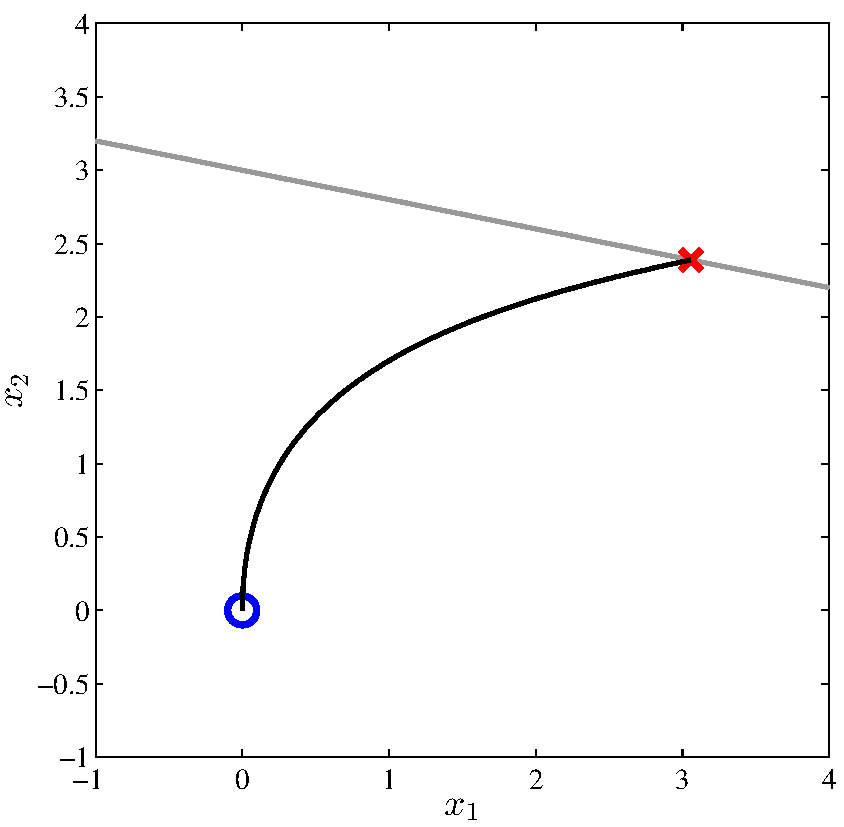
\includegraphics[width=3in]{\figurepath/prob2.pdf}
    \caption{State history with optimal control input to get from the origin $(0,0)$ to the line $x_{1}(t)+5x_{2}(t)=15$\label{fig:prob2}}
  \end{figure}

  \clearpage
  \section{Special Cases Including the Beltrami Identity}

  In the calculus of variations problem, where the goal is to minimize

  \begin{equation*}
    J=\int_{t_{0}}^{t_{f}}g(x,\dot{x},t)dt
  \end{equation*}

  we showed that the first order necessary condition is

  \begin{equation*}
    \frac{\partial{}g}{\partial{}x}-\frac{d}{dt}\biggr\{\frac{\partial{}g}{\partial\dot{x}}\biggr\}=0
  \end{equation*}

  subject to various (assumed to be well defined) initial and terminal conditions, depending on the problem statement.
  Now consider the following:

  \begin{enumerate}
    \item{If we can write $g\rightarrow g(\dot{x})$ (i.e., the function $g$ is not an explicit function of $x$ or $t$), show that there always exists a solution that is a linear function of time.}
    \item{If we can write $g\rightarrow g(x,\dot{x})$ (i.e., the function $g$ is not an explicit function of time), show that}
    \begin{equation*}
      g-\dot{x}\frac{\partial{}g}{\partial\dot{x}}=\text{constant}
    \end{equation*}
  \end{enumerate}

  \subsection*{Answer}
  \subsubsection*{Part 1}

  Let $x(t)=a_{1}t+a_{2}$ a linear function of time.
  Then $\dot{x}(t)=a_{1}$ is constant.
  With $g=g(\dot{x})$ the Euler-Lagrange equation reduces to

  \begin{equation*}
    \frac{d}{dt}\biggr\{\frac{\partial{}g}{\partial\dot{x}}\biggr\}=0
  \end{equation*}

  Making the substituting $f(\dot{x})=\frac{\partial{}g}{\partial\dot{x}}$ we have $\frac{d}{dt}f(\dot{x})=0$ to which we can apply the chain rule to get $\frac{d}{dt}f(\dot{x})=\frac{\partial{}f}{\partial\dot{x}}\frac{d\dot{x}}{dt}=\frac{\partial{}f}{\partial\dot{x}}\ddot{x}=0$.
  Substituting back in for $f(\dot{x})$ we get

  \begin{equation*}
    \frac{\partial^{2}g}{\partial\dot{x}^{2}}\ddot{x}=0
  \end{equation*}

  With $x$ a linear function of time, $\ddot{x}$ is zero, thus satisfying the first order necessary condition.

  \subsubsection*{Part 2}

  First evaluate the full derivative of $g$ with respect to time.

  \begin{equation*}
    \frac{dg}{dt}=\frac{\partial{}g}{\partial{}x}\frac{\partial{}x}{\partial{}t}+\frac{\partial{}g}{\partial\dot{x}}\frac{\partial\dot{x}}{\partial{}t}+\frac{\partial{}g}{\partial{}t}
  \end{equation*}

  Rearrange this to obtain

  \begin{equation*}
    \frac{\partial{}g}{\partial{}x}\frac{\partial{}x}{\partial{}t}=
    \frac{dg}{dt}-\frac{\partial{}g}{\partial\dot{x}}\frac{\partial\dot{x}}{\partial{}t}-\frac{\partial{}g}{\partial{}t}
  \end{equation*}

  Now multiply the Euler-Lagrange equation through by $\frac{\partial{}x}{\partial{}t}$

  \begin{equation*}
    \frac{\partial{}g}{\partial{}x}\frac{\partial{}x}{\partial{}t}-\frac{d}{dt}\biggr\{\frac{\partial{}g}{\partial\dot{x}}\biggr\}\frac{\partial{}x}{\partial{}t}=0
  \end{equation*}

  rearranging

  \begin{equation*}
    \frac{\partial{}g}{\partial{}x}\frac{\partial{}x}{\partial{}t}=\frac{d}{dt}\biggr\{\frac{\partial{}g}{\partial\dot{x}}\biggr\}\frac{\partial{}x}{\partial{}t}
  \end{equation*}

  Using our identity from before and plugging it in

  \begin{equation*}
    \frac{dg}{dt}-\frac{\partial{}g}{\partial\dot{x}}\frac{\partial\dot{x}}{\partial{}t}-\frac{\partial{}g}{\partial{}t}=\frac{d}{dt}\biggr\{\frac{\partial{}g}{\partial\dot{x}}\biggr\}\frac{\partial{}x}{\partial{}t}
  \end{equation*}

  Rearranging

  \begin{equation*}
  -\frac{\partial{}g}{\partial{}t}+\frac{dg}{dt}-\frac{\partial{}g}{\partial\dot{x}}\frac{\partial\dot{x}}{\partial{}t}-\frac{d}{dt}\biggr\{\frac{\partial{}g}{\partial\dot{x}}\biggr\}\frac{\partial{}x}{\partial{}t}=0
  \end{equation*}

  Recognize by product rule that

  \begin{align*}
    \frac{d}{dt}\biggr(\frac{\partial{}x}{\partial{}t}\frac{\partial{}g}{\partial\dot{x}}\biggr)&=
    \frac{d}{dt}\left(\frac{\partial{}x}{\partial{}t}\right)\frac{\partial{}g}{\partial\dot{x}}+\frac{\partial{}x}{\partial{}t}\frac{d}{dt}\biggr(\frac{\partial{}g}{\partial\dot{x}}\biggr) \\
    &=\frac{\partial{}g}{\partial\dot{x}}\frac{\partial\dot{x}}{\partial{}t}+\frac{d}{dt}\biggr(\frac{\partial{}g}{\partial\dot{x}}\biggr)\frac{\partial{}x}{\partial{}t}
  \end{align*}

  This allows us to rewrite the above as

  \begin{equation*}
    -\frac{\partial{}g}{\partial{}t}+\frac{dg}{dt}-\frac{d}{dt}\biggr(\frac{\partial{}x}{\partial{}t}\frac{\partial{}g}{\partial\dot{x}}\biggr)=0
  \end{equation*}

  which we can simplify as

  \begin{equation*}
    -\frac{\partial{}g}{\partial{}t}+\frac{d}{dt}\biggr(g-\frac{\partial{}x}{\partial{}t}\frac{\partial{}g}{\partial\dot{x}}\biggr)=0
  \end{equation*}

  With the given condition that $g$ is not an explicit function of time, $\frac{\partial{}g}{\partial{}t}=0$ and the above reduces to

  \begin{equation*}
    \frac{d}{dt}\biggr(g-\frac{\partial{}x}{\partial{}t}\frac{\partial{}g}{\partial\dot{x}}\biggr)=0
  \end{equation*}

  and so

  \begin{equation*}
    \boxed{%
      g-\dot{x}\frac{\partial{}g}{\partial\dot{x}}=\text{constant}
    }
  \end{equation*}

  which is the desired result.

  \clearpage
  \section{Integral/Isoperimetric Constraints}

  One important calculus of variations problem that we did not discuss in class has the same basic form, but with constraints that are given by an integral, called isoperimetric constraints:

  \begin{equation*}
    J=\int_{t_{0}}^{t_{f}}g(x,\dot{x},t)dt
  \end{equation*}

  such that

  \begin{equation*}
    \int_{t_{0}}^{t_{f}}e(x,\dot{x},t)dt=C
  \end{equation*}

  where we will assume that $t_{f}$ is free but $x(t_{f})$ is fixed.

  \begin{enumerate}
    \item{%
      Use the same approach followed in the notes to find the necessary and boundary conditions for this optimal control problem.
      In particular, augment the constraint to the cost using a constant Lagrange Multiplier vector $\nu$, and show that these conditions can be written in the form
    }
    \begin{align*}
      \frac{\partial{}g_{a}}{\partial{}x}-\frac{d}{dt}\biggr\{\frac{\partial{}g_{a}}{\partial\dot{x}}\biggr\}&=0 \\
      g_{a}(t_{f})-\frac{\partial{}g_{a}}{\partial\dot{x}}(t_{f})\dot{x}(t_{f})&=0 \\
      \int_{t_{0}}^{t_{f}}e(x,\dot{x},t)dt&=C
    \end{align*}

    where $g_{a}=g+\nu^{\top}e$.

    \item{%
      Use the results of part 1 to clearly state the differential equations and corresponding boundary conditions that must be solved to find the curve $y(x)$ of a specified length $L$ with endpoints on the $x-$axis (i.e., so that $y(0)=y(x_{f})=0$) that encloses the maximum area.
      That is, maximize
    }

    \begin{equation*}
      J=\int_{0}^{x_{f}}y(x)dx
    \end{equation*}

    subject to

    \begin{equation*}
      \int_{0}^{x_{f}}\sqrt{1+y'(x)^{2}}dx=L
    \end{equation*}

    where $x_{f}$ is free.
  \end{enumerate}

  \subsection*{Answer}
  \subsubsection*{Part 1}

  First augment the given cost with a Lagrange multiplier and the constraint and define this as $J_{a}(x)$

  \begin{equation*}
    J_{a}(x)=\int_{t_{0}}^{t_{f}}g(x,\dot{x},t)dt+\nu^{\top}\biggr(\int_{t_{0}}^{t_{f}}e(x,\dot{x},t)dt-C\biggr)
  \end{equation*}

  Now we will calculate the increment and from there the first variation by taking linear terms in the increment.
  The Increment is given by $\Delta J_{a}=J_{a}(x+\delta x)-J_{a}(x)$.
  First evaluate $J_{a}(x+\delta x)$ as

  \begin{equation*}
    J_{a}(x+\delta x)=
    \int_{t_{0}+\delta t_{0}}^{t_{f}+\delta t_{f}}g(x+\delta x,\dot{x}+\delta\dot{x},t)dt+(\nu+\delta\nu)^{\top}\biggr(\int_{t_{0}+\delta t_{0}}^{t_{f}+\delta t_{f}}e(x+\delta x,\dot{x}+\delta\dot{x},t)dt-C\biggr)
  \end{equation*}

  To simplify this expression, begin by splitting the integrals into three pieces as

  \begin{align*}
    J_{a}(x+\delta x)&=
    \int_{t_{0}}^{t_{f}}g(x+\delta x,\dot{x}+\delta\dot{x},t)dt
    +(\nu+\delta\nu)^{\top}\biggr(\int_{t_{0}}^{t_{f}}e(x+\delta x,\dot{x}+\delta\dot{x},t)dt-C\biggr) \\
    &+
    \int_{t_{0}+\delta t_{0}}^{t_{0}}g(x+\delta x,\dot{x}+\delta\dot{x},t)dt+
    \int_{t_{f}}^{t_{f}+\delta t_{f}}g(x+\delta x,\dot{x}+\delta\dot{x},t)dt \\
    &+(\nu+\delta\nu)^{\top}\biggr(
    \int_{t_{0}+\delta t_{0}}^{t_{0}}e(x+\delta x,\dot{x}+\delta\dot{x},t)dt+
    \int_{t_{f}}^{t_{f}+\delta t_{f}}e(x+\delta x,\dot{x}+\delta\dot{x},t)dt\biggr)
  \end{align*}

  Then flip the limits of integration on one of the integrals and put a minus sign out front.

  \begin{align*}
    J_{a}(x+\delta x)&=
    \int_{t_{0}}^{t_{f}}g(x+\delta x,\dot{x}+\delta\dot{x},t)dt
    +(\nu+\delta\nu)^{\top}\biggr(\int_{t_{0}}^{t_{f}}e(x+\delta x,\dot{x}+\delta\dot{x},t)dt-C\biggr) \\
    &-
    \int_{t_{0}}^{t_{0}+\delta t_{0}}g(x+\delta x,\dot{x}+\delta\dot{x},t)dt+
    \int_{t_{f}}^{t_{f}+\delta t_{f}}g(x+\delta x,\dot{x}+\delta\dot{x},t)dt \\
    &+(\nu+\delta\nu)^{\top}\biggr(
    -\int_{t_{0}}^{t_{0}+\delta t_{0}}e(x+\delta x,\dot{x}+\delta\dot{x},t)dt+
    \int_{t_{f}}^{t_{f}+\delta t_{f}}e(x+\delta x,\dot{x}+\delta\dot{x},t)dt\biggr)
  \end{align*}

  Next, since these ``end regions'' are being integrated over a small distance $\delta t$, we can approximate the integrals using $\int_{t}^{t+\delta t}f(\tau)d\tau=f(t)\delta t$.
  This gives

  \begin{align*}
    J_{a}(x+\delta x)&=
    \int_{t_{0}}^{t_{f}}g(x+\delta x,\dot{x}+\delta\dot{x},t)dt
    +(\nu+\delta\nu)^{\top}\biggr(\int_{t_{0}}^{t_{f}}e(x+\delta x,\dot{x}+\delta\dot{x},t)dt-C\biggr) \\
    &-g(x+\delta x,\dot{x}+\delta\dot{x},t)\bigr|_{t_{0}}\delta t_{0}
    +g(x+\delta x,\dot{x}+\delta\dot{x},t)\bigr|_{t_{f}}\delta t_{f} \\
    &+(\nu+\delta\nu)^{\top}\biggr(
    -e(x+\delta x,\dot{x}+\delta\dot{x},t)\bigr|_{t_{0}}\delta t_{0}
    +e(x+\delta x,\dot{x}+\delta\dot{x},t)\bigr|_{t_{f}}\delta t_{f}
    \biggr)
  \end{align*}

  Now perform a Taylor series expansion of some of the functions, neglecting terms with order greater than linear.
  This is the first step of simplifying the increment to the first variation, as we are only retaining linear terms.
  These Taylor series approximations are

  \begin{align*}
    g(x+\delta x,\dot{x}+\delta\dot{x},t)&\approx g(x,\dot{x},t)+\frac{\partial{}g}{\partial{}x}\delta x+\frac{\partial{}g}{\partial\dot{x}}\delta\dot{x} \\
    e(x+\delta x,\dot{x}+\delta\dot{x},t)&\approx e(x,\dot{x},t)+\frac{\partial{}e}{\partial{}x}\delta x+\frac{\partial{}e}{\partial\dot{x}}\delta\dot{x}
  \end{align*}

  Plugging the Taylor series approximations in we get

  \begin{align*}
    J_{a}(x+\delta x)&\approx
    \int_{t_{0}}^{t_{f}}\biggr\{g(x,\dot{x},t)+\frac{\partial{}g}{\partial{}x}\delta x+\frac{\partial{}g}{\partial\dot{x}}\delta\dot{x}\biggr\}dt
    +(\nu+\delta\nu)^{\top}\biggr(\int_{t_{0}}^{t_{f}}\biggr\{e(x,\dot{x},t)+\frac{\partial{}e}{\partial{}x}\delta x+\frac{\partial{}e}{\partial\dot{x}}\delta\dot{x}\biggr\}dt-C\biggr) \\
    &-\biggr\{g(x,\dot{x},t)+\frac{\partial{}g}{\partial{}x}\delta x+\frac{\partial{}g}{\partial\dot{x}}\delta\dot{x}\biggr\}\biggr|_{t_{0}}\delta t_{0}
    +\biggr\{g(x,\dot{x},t)+\frac{\partial{}g}{\partial{}x}\delta x+\frac{\partial{}g}{\partial\dot{x}}\delta\dot{x}\biggr\}\biggr|_{t_{f}}\delta t_{f} \\
    &+(\nu+\delta\nu)^{\top}\biggr(
    -\biggr\{e(x,\dot{x},t)+\frac{\partial{}e}{\partial{}x}\delta x+\frac{\partial{}e}{\partial\dot{x}}\delta\dot{x}\biggr\}\biggr|_{t_{0}}\delta t_{0}
    +\biggr\{e(x,\dot{x},t)+\frac{\partial{}e}{\partial{}x}\delta x+\frac{\partial{}e}{\partial\dot{x}}\delta\dot{x}\biggr\}\biggr|_{t_{f}}\delta t_{f}
    \biggr)
  \end{align*}

  And now we continue to simplify by eliminating any other terms that are higher than first order terms.

  \begin{align*}
    J_{a}(x+\delta x)&\approx
    \int_{t_{0}}^{t_{f}}\biggr\{g(x,\dot{x},t)+\frac{\partial{}g}{\partial{}x}\delta x+\frac{\partial{}g}{\partial\dot{x}}\delta\dot{x}\biggr\}dt
    +(\nu+\delta\nu)^{\top}\biggr(\int_{t_{0}}^{t_{f}}\biggr\{e(x,\dot{x},t)+\frac{\partial{}e}{\partial{}x}\delta x+\frac{\partial{}e}{\partial\dot{x}}\delta\dot{x}\biggr\}dt-C\biggr) \\
    &-g(x,\dot{x},t)\biggr|_{t_{0}}\delta t_{0}
    +g(x,\dot{x},t)\biggr|_{t_{f}}\delta t_{f}
    +\nu^{\top}\biggr(
    -e(x,\dot{x},t)\biggr|_{t_{0}}\delta t_{0}
    +e(x,\dot{x},t)\biggr|_{t_{f}}\delta t_{f}
    \biggr)
  \end{align*}

  Continuing to simplify by expanding the $(\nu+\delta\nu)^{\top}$ term

  \begin{align*}
    J_{a}(x+\delta x)&\approx
    \int_{t_{0}}^{t_{f}}\biggr\{g(x,\dot{x},t)+\frac{\partial{}g}{\partial{}x}\delta x+\frac{\partial{}g}{\partial\dot{x}}\delta\dot{x}\biggr\}dt
    +\nu\biggr(\int_{t_{0}}^{t_{f}}\biggr\{e(x,\dot{x},t)+\frac{\partial{}e}{\partial{}x}\delta x+\frac{\partial{}e}{\partial\dot{x}}\delta\dot{x}\biggr\}dt-C\biggr) \\
    &+\delta\nu^{\top}\int_{t_{0}}^{t_{f}}\biggr\{e(x,\dot{x},t)+\frac{\partial{}e}{\partial{}x}\delta x+\frac{\partial{}e}{\partial\dot{x}}\delta\dot{x}\biggr\}dt-\delta\nu^{\top}C \\
    &-g(x,\dot{x},t)\biggr|_{t_{0}}\delta t_{0}
    +g(x,\dot{x},t)\biggr|_{t_{f}}\delta t_{f}
    +\nu^{\top}\biggr(
    -e(x,\dot{x},t)\biggr|_{t_{0}}\delta t_{0}
    +e(x,\dot{x},t)\biggr|_{t_{f}}\delta t_{f}
    \biggr)
  \end{align*}

  Continue simplifying by eliminating terms

  \begin{align*}
    J_{a}(x+\delta x)&\approx
    \int_{t_{0}}^{t_{f}}\biggr\{g(x,\dot{x},t)+\frac{\partial{}g}{\partial{}x}\delta x+\frac{\partial{}g}{\partial\dot{x}}\delta\dot{x}\biggr\}dt
    +\nu^{\top}\biggr(\int_{t_{0}}^{t_{f}}\biggr\{e(x,\dot{x},t)+\frac{\partial{}e}{\partial{}x}\delta x+\frac{\partial{}e}{\partial\dot{x}}\delta\dot{x}\biggr\}dt-C\biggr) \\
    &+\delta\nu^{\top}\int_{t_{0}}^{t_{f}}e(x,\dot{x},t)dt-\delta\nu^{\top}C \\
    &-g(x,\dot{x},t)\biggr|_{t_{0}}\delta t_{0}
    +g(x,\dot{x},t)\biggr|_{t_{f}}\delta t_{f}
    +\nu^{\top}\biggr(
    -e(x,\dot{x},t)\biggr|_{t_{0}}\delta t_{0}
    +e(x,\dot{x},t)\biggr|_{t_{f}}\delta t_{f}
    \biggr)
  \end{align*}

  Now recall the following.
  To calculate the variation, we subtract the following from our expression above.

  \begin{equation*}
    J_{a}(x)=\int_{t_{0}}^{t_{f}}g(x,\dot{x},t)dt+\nu^{\top}\biggr(\int_{t_{0}}^{t_{f}}e(x,\dot{x},t)dt-C\biggr)
  \end{equation*}

  Subtracting these two to get the variation which is the increment approximated to first order

  \begin{align*}
    \delta J_{a}(x,\delta x)&=
    \int_{t_{0}}^{t_{f}}\biggr\{\frac{\partial{}g}{\partial{}x}\delta x+\frac{\partial{}g}{\partial\dot{x}}\delta\dot{x}\biggr\}dt
    +\nu^{\top}\int_{t_{0}}^{t_{f}}\biggr\{\frac{\partial{}e}{\partial{}x}\delta x+\frac{\partial{}e}{\partial\dot{x}}\delta\dot{x}\biggr\}dt \\
    &+\delta\nu^{\top}\int_{t_{0}}^{t_{f}}e(x,\dot{x},t)dt-\delta\nu^{\top}C \\
    &-g(x,\dot{x},t)\biggr|_{t_{0}}\delta t_{0}
    +g(x,\dot{x},t)\biggr|_{t_{f}}\delta t_{f}
    +\nu^{\top}\biggr(
    -e(x,\dot{x},t)\biggr|_{t_{0}}\delta t_{0}
    +e(x,\dot{x},t)\biggr|_{t_{f}}\delta t_{f}
    \biggr)
  \end{align*}

  Simplify this expression by combining the integrals

  \begin{align*}
    \delta J_{a}(x,\delta x)&=
    \int_{t_{0}}^{t_{f}}\biggr(\biggr\{\frac{\partial{}g}{\partial{}x}\delta x+\frac{\partial{}g}{\partial\dot{x}}\delta\dot{x}\biggr\}
    +\nu^{\top}\biggr\{\frac{\partial{}e}{\partial{}x}\delta x+\frac{\partial{}e}{\partial\dot{x}}\delta\dot{x}\biggr\}\biggr)dt \\
    &+\delta\nu^{\top}\int_{t_{0}}^{t_{f}}e(x,\dot{x},t)dt-\delta\nu^{\top}C \\
    &-g(x,\dot{x},t)\biggr|_{t_{0}}\delta t_{0}
    +g(x,\dot{x},t)\biggr|_{t_{f}}\delta t_{f}
    +\nu^{\top}\biggr(
    -e(x,\dot{x},t)\biggr|_{t_{0}}\delta t_{0}
    +e(x,\dot{x},t)\biggr|_{t_{f}}\delta t_{f}
    \biggr)
  \end{align*}

  Further simplifying the first integral using linearity of the derivative operator we have

  \begin{align*}
    \delta J_{a}(x,\delta x)&=
    \int_{t_{0}}^{t_{f}}\biggr\{\frac{\partial(g+\nu^{\top}e)}{\partial{}x}\delta x+\frac{\partial(g+\nu^{\top}e)}{\partial\dot{x}}\delta\dot{x}\biggr\}dt
    +\delta\nu^{\top}\biggr(\int_{t_{0}}^{t_{f}}e(x,\dot{x},t)dt-C\biggr) \\
    &-\biggr\{g(x,\dot{x},t)+\nu^{\top}e(x,\dot{x},t)\biggr\}\biggr|_{t_{0}}\delta t_{0}
    +\biggr\{g(x,\dot{x},t)+\nu^{\top}e(x,\dot{x},t)\biggr\}\biggr|_{t_{f}}\delta t_{f}
  \end{align*}

  Simplifying more using the notation $g_{a}=g+\nu^{\top}e$ we get

  \begin{align*}
    \delta J_{a}(x,\delta x)&=
    \int_{t_{0}}^{t_{f}}\biggr\{\frac{\partial{}g_{a}}{\partial{}x}\delta x+\frac{\partial{}g_{a}}{\partial\dot{x}}\delta\dot{x}\biggr\}dt
    +\delta\nu^{\top}\biggr(\int_{t_{0}}^{t_{f}}e(x,\dot{x},t)dt-C\biggr) \\
    &+g_{a}(x,\dot{x},t)\biggr|_{t_{f}}\delta t_{f}
    -g_{a}(x,\dot{x},t)\biggr|_{t_{0}}\delta t_{0}
  \end{align*}

  Now we need to integrate the first term by parts, but we will split the integral into two parts and only integrate the second integrand by parts, so we will look at just that term

  \begin{equation*}
    \int_{t_{0}}^{t_{f}}\frac{\partial{}g_{a}}{\partial\dot{x}}\delta\dot{x}dt
  \end{equation*}

  let

  \begin{align*}
    u&=\frac{\partial{}g_{a}}{\partial\dot{x}} \\
    dv&=\delta\dot{x}dt
  \end{align*}

  which gives

  \begin{align*}
    du&=\frac{d}{dt}\frac{\partial{}g_{a}}{\partial\dot{x}} \\
    v&=\delta x
  \end{align*}

  Now use

  \begin{equation*}
    \int udv=uv-\int vdu
  \end{equation*}

  and get

  \begin{equation*}
    \int \frac{\partial{}g_{a}}{\partial\dot{x}}\delta\dot{x}dt
    =
    \frac{\partial{}g_{a}}{\partial\dot{x}}\delta x
    -\int\delta x\frac{d}{dt}\frac{\partial{}g_{a}}{\partial\dot{x}}
  \end{equation*}

  Plugging this result back into the equation for the variation we get

  \begin{align*}
    \delta J_{a}(x,\delta x)&=
    \int_{t_{0}}^{t_{f}}\biggr\{\frac{\partial{}g_{a}}{\partial{}x}\delta x-\delta x\frac{d}{dt}\frac{\partial{}g_{a}}{\partial\dot{x}}\biggr\}dt
    +\frac{\partial{}g_{a}}{\partial\dot{x}}\delta x\biggr|_{t_{0}}^{t_{f}}
    +\delta\nu^{\top}\biggr(\int_{t_{0}}^{t_{f}}e(x,\dot{x},t)dt-C\biggr) \\
    &+g_{a}(x,\dot{x},t)\biggr|_{t_{f}}\delta t_{f}
    -g_{a}(x,\dot{x},t)\biggr|_{t_{0}}\delta t_{0}
  \end{align*}

  Simplifying some more we can pull the $\delta x$ term out of the brackets in the first integral and splitting up the boundary conditions term

  \begin{align*}
    \delta J_{a}(x,\delta x)&=
    \int_{t_{0}}^{t_{f}}\biggr\{\frac{\partial{}g_{a}}{\partial{}x}-\frac{d}{dt}\frac{\partial{}g_{a}}{\partial\dot{x}}\biggr\}\delta xdt
    +\delta\nu^{\top}\biggr(\int_{t_{0}}^{t_{f}}e(x,\dot{x},t)dt-C\biggr) \\
    &+g_{a}(x,\dot{x},t)\biggr|_{t_{f}}\delta t_{f}
    -g_{a}(x,\dot{x},t)\biggr|_{t_{0}}\delta t_{0}
    +\frac{\partial{}g_{a}}{\partial\dot{x}}\delta x\biggr|_{t_{f}}
    -\frac{\partial{}g_{a}}{\partial\dot{x}}\delta x\biggr|_{t_{0}}
  \end{align*}

  But now we need to simplify $\delta x(t_{0})$ and $\delta x(t_{f})$ as follows.
  This can be most easily seen by drawing a picture of the two curves $J(x)$ and $J(x+\delta x)$.

  \begin{align*}
    \delta x(t_{0})&\approx\delta x_{0}-\dot{x}(t_{0})\delta t_{0} \\
    \delta x(t_{f})&\approx\delta x_{f}-\dot{x}(t_{f})\delta t_{f}
  \end{align*}

  Substituting this simplification in $\delta J_{a}$ becomes

  \begin{align*}
    \delta J_{a}(x,\delta x)&=
    \int_{t_{0}}^{t_{f}}\biggr\{\frac{\partial{}g_{a}}{\partial{}x}-\frac{d}{dt}\frac{\partial{}g_{a}}{\partial\dot{x}}\biggr\}\delta xdt
    +\delta\nu^{\top}\biggr(\int_{t_{0}}^{t_{f}}e(x,\dot{x},t)dt-C\biggr) \\
    &+g_{a}(x,\dot{x},t)\biggr|_{t_{f}}\delta t_{f}
    -g_{a}(x,\dot{x},t)\biggr|_{t_{0}}\delta t_{0}
    +\frac{\partial{}g_{a}}{\partial\dot{x}}\biggr|_{t_{f}}\biggr(\delta x_{f}-\dot{x}(t_{f})\delta t_{f}\biggr)
    -\frac{\partial{}g_{a}}{\partial\dot{x}}\biggr|_{t_{0}}\biggr(\delta x_{0}-\dot{x}(t_{0})\delta t_{0}\biggr)
  \end{align*}

  Now we can simplify the notation a little bit and group terms

  \begin{align*}
    \delta J_{a}(x,\delta x)&=
    \int_{t_{0}}^{t_{f}}\biggr\{\frac{\partial{}g_{a}}{\partial{}x}-\frac{d}{dt}\frac{\partial{}g_{a}}{\partial\dot{x}}\biggr\}\delta xdt
    +\delta\nu^{\top}\biggr(\int_{t_{0}}^{t_{f}}e(x,\dot{x},t)dt-C\biggr) \\
    &+g_{a}(t_{f})\delta t_{f}
    -g_{a}(t_{0})\delta t_{0}
    +\frac{\partial{}g_{a}}{\partial\dot{x}}\biggr|_{t_{f}}\delta x_{f}
    -\frac{\partial{}g_{a}}{\partial\dot{x}}\biggr|_{t_{f}}\dot{x}(t_{f})\delta t_{f}
    -\frac{\partial{}g_{a}}{\partial\dot{x}}\biggr|_{t_{0}}\delta x_{0}
    +\frac{\partial{}g_{a}}{\partial\dot{x}}\biggr|_{t_{0}}\dot{x}(t_{0})\delta t_{0}
  \end{align*}

  Finally grouping the last of the like terms together we get

  \begin{empheq}[box=\fbox]{alignat*=3}
    \delta{}J_{a}(x,\delta{}x)&=
    \int_{t_{0}}^{t_{f}}\biggr\{\frac{\partial{}g_{a}}{\partial{}x}-\frac{d}{dt}\frac{\partial{}g_{a}}{\partial\dot{x}}\biggr\}\delta{}xdt
    +\delta\nu^{\top}\biggr(\int_{t_{0}}^{t_{f}}e(x,\dot{x},t)dt-C\biggr) \\
    &+\biggr(g_{a}(t_{f})-\frac{\partial{}g_{a}}{\partial\dot{x}}\biggr|_{t_{f}}\dot{x}(t_{f})\biggr)\delta{}t_{f}
    -\biggr(g_{a}(t_{0})-\frac{\partial{}g_{a}}{\partial\dot{x}}\biggr|_{t_{0}}\dot{x}(t_{0})\biggr)\delta{}t_{0}
    +\frac{\partial{}g_{a}}{\partial\dot{x}}\biggr|_{t_{f}}\delta{}x_{f}
    -\frac{\partial{}g_{a}}{\partial\dot{x}}\biggr|_{t_{0}}\delta{}x_{0}
  \end{empheq}

  And now we can simplify this general expression using the given boundary conditions and find the desired necessary conditions.
  We have $\delta x_{f}=0$, $\delta t_{0}=0$, and $\delta x_{0}=0$ reducing the above to

  \begin{align*}
    \delta J_{a}(x,\delta x)&=
    \int_{t_{0}}^{t_{f}}\biggr\{\frac{\partial{}g_{a}}{\partial{}x}-\frac{d}{dt}\frac{\partial{}g_{a}}{\partial\dot{x}}\biggr\}\delta xdt
    +\delta\nu^{\top}\biggr(\int_{t_{0}}^{t_{f}}e(x,\dot{x},t)dt-C\biggr) \\
    &+\biggr(g_{a}(t_{f})-\frac{\partial{}g_{a}}{\partial\dot{x}}\biggr|_{t_{f}}\dot{x}(t_{f})\biggr)\delta t_{f}
  \end{align*}

  And since this has to hold for all $\delta x$, as well as the fact that $\delta t_{f}$ is not zero and $\delta\nu^{\top}$ is not zero, the necessary conditions are

  \begin{empheq}[box=\fbox]{alignat*=3}
    \frac{\partial{}g_{a}}{\partial{}x}-\frac{d}{dt}\bigg\{\frac{\partial{}g_{a}}{\partial\dot{x}}\biggr\}&=0 \\
    \int_{t_{0}}^{t_{f}}e(x,\dot{x},t)dt-C&=0 \\
    g_{a}(t_{f})-\frac{\partial{}g_{a}}{\partial\dot{x}}\biggr|_{t_{f}}\dot{x}(t_{f})&=0
  \end{empheq}

  As desired.

  \subsubsection*{Part 2}

  Using the results of Part 1 form the augmented function $g_{a}$ as $g_{a}=g+\nu e$ where $g=y(x)$ and $e=\sqrt{1+y'(x)^{2}}$ giving

  \begin{equation*}
    y_{a}(x,\dot{x})=y(x)+\nu\sqrt{1+y'(x)^{2}}
  \end{equation*}

  The Euler-Lagrange equation becomes

  \begin{equation*}
    \frac{\partial{}g_{a}}{\partial{}y}-\frac{d}{dx}\bigg\{\frac{\partial{}y_{a}}{\partial{}y'}\biggr\}=0
  \end{equation*}

  Evaluating $\frac{\partial{}y_{a}}{\partial{}y'}$ we have

  \begin{equation*}
    \frac{\partial{}y_{a}}{\partial{}y'}=
    \frac{\lambda y'(x)}{\sqrt{1+y'(x)^{2}}}
  \end{equation*}

  Plugging this in

  \begin{equation*}
    1-\frac{d}{dx}\bigg\{\frac{\lambda y'(x)}{\sqrt{1+y'(x)^{2}}}\biggr\}=0
  \end{equation*}

  Now evaluate the following derivative using product rule

  \begin{equation*}
    \frac{d}{dx}\bigg\{\frac{\lambda y'(x)}{\sqrt{1+y'(x)^{2}}}\biggr\}=
    \frac{d}{dx}(\lambda y'(x))\frac{1}{\sqrt{1+y'(x)^{2}}}+
    \lambda y'(x)\frac{d}{dx}\biggr(\frac{1}{\sqrt{1+y'(x)^{2}}}\biggr)
  \end{equation*}

  Evaluating the second term on the right hand side

  \begin{align*}
    \frac{d}{dx}\biggr(\frac{1}{\sqrt{1+y'(x)^{2}}}\biggr)&=
    \frac{d}{dx}\biggr(1+\biggr(\frac{\partial{}y}{\partial{}x}\biggr)^{2}\biggr)^{-\frac{1}{2}} \\
    &=-\frac{1}{2}\biggr(1+\biggr(\frac{\partial{}y}{\partial{}x}\biggr)^{2}\biggr)^{-\frac{3}{2}}\cdot 2\biggr(\frac{\partial{}y}{\partial{}x}\biggr)\frac{\partial^{2}y}{\partial{}x^{2}} \\
    &=-\frac{\bigr(\frac{\partial{}y}{\partial{}x}\bigr)\frac{\partial^{2}y}{\partial{}x^{2}}}{\bigr(1+\bigr(\frac{\partial{}y}{\partial{}x}\bigr)^{2}\bigr)^{\frac{3}{2}}}
  \end{align*}

  Then our derivative from the Euler-Lagrange equation becomes

  \begin{align*}
    \frac{d}{dx}\bigg\{\frac{\lambda y'(x)}{\sqrt{1+y'(x)^{2}}}\biggr\}&=
    \frac{\lambda\frac{\partial^{2}y}{\partial{}x^{2}}}{\sqrt{1+y'(x)^{2}}}-
    \frac{\lambda\frac{\partial{}y}{\partial{}x}\bigr(\frac{\partial{}y}{\partial{}x}\bigr)\frac{\partial^{2}y}{\partial{}x^{2}}}{\bigr(1+\bigr(\frac{\partial{}y}{\partial{}x}\bigr)^{2}\bigr)^{\frac{3}{2}}} \\
    &=\frac{\lambda\frac{\partial^{2}y}{\partial{}x^{2}}(1+\bigr(\frac{\partial{}y}{\partial{}x}\bigr)^{2})-\lambda\bigr(\frac{\partial{}y}{\partial{}x}\bigr)^{2}\frac{\partial^{2}y}{\partial{}x^{2}}}{\bigr(1+\bigr(\frac{\partial{}y}{\partial{}x}\bigr)^{2})^{\frac{3}{2}}} \\
    &=\frac{\lambda\frac{\partial^{2}y}{\partial{}x^{2}}}{\bigr(1+\bigr(\frac{\partial{}y}{\partial{}x}\bigr)^{2}\bigr)^{\frac{3}{2}}} \\
  \end{align*}

  So the Euler-Lagrange equation is

  \begin{equation*}
    \boxed{%
      1-\frac{\lambda\frac{\partial^{2}y}{\partial{}x^{2}}}{\bigr(1+\bigr(\frac{\partial{}y}{\partial{}x}\bigr)^{2}\bigr)^{\frac{3}{2}}}=0
    }
  \end{equation*}

  The boundary conditions are

  \begin{empheq}[box=\fbox]{alignat*=3}
    \int_{0}^{x_{f}}\sqrt{1+y'(x)^{2}}dx-L&=0 \\
    y_{a}(x_{f})-\frac{\partial{}y_{a}}{\partial{}y'}\biggr|_{x_{f}}y'(x_{f})&=0
  \end{empheq}

  \subsubsection*{Part 3}

  The solution $y$ we expect to be a circle, or half circle in this case.
  That is it will take the form

  \begin{equation*}
    y=\sqrt{r^{2}-\biggr(x-\frac{1}{2}\biggr)^{2}}+c
  \end{equation*}

  Plugging this into the Euler-Lagrange equation above, we can see that it is satisfied, and we only need to apply boundary conditions to determine the values of the constants $r$ and $c$.

  \clearpage
  \section{LQR Control}

  Consider the system with dynamics

  \begin{align*}
    \dot{x}=
    \begin{bmatrix}
      0 & 1 \\
      -6 & -5
    \end{bmatrix}
    x+
    \begin{bmatrix}
      0 \\
      1
    \end{bmatrix}
    u \\
    z&=
    \begin{bmatrix}
      1 & 1
    \end{bmatrix}x
  \end{align*}

  and cost function

  \begin{equation*}
    J=\frac{1}{2}\int_{0}^{\infty}\bigr(z^{2}(t)+\rho u^{2}(t)\bigr)dt
  \end{equation*}

  \begin{enumerate}
    \item{Find the control law $u(t)=-Fx(t)$ that minimizes the cost, for $\rho=0.01$.}
    \item{Plot the closed-loop response $z(t)$ and control input $u(t)$ for the initial conditions $x_{1}(0)=1$, $x_{2}(0)=0$.}
    \item{Repeat parts (1) and (2) for the system}
    \begin{align*}
      \dot{x}=
      \begin{bmatrix}
        0 & 1 \\
        -6 & -5
      \end{bmatrix}
      x+
      \begin{bmatrix}
        0 \\
        1
      \end{bmatrix}
      u \\
      z&=
      \begin{bmatrix}
        1 & 1
      \end{bmatrix}x
    \end{align*}
    with the same cost function.
    \item{Which system has better closed-loop performance? Explain why.}
  \end{enumerate}

  \subsection*{Answer}

  From the cost function we have

  \begin{equation*}
    R_{zz}=1
    \qquad
    R_{xx}=
    \begin{bmatrix}
      1 & 1 \\
      1 & 1
    \end{bmatrix}
  \end{equation*}

  We form the Hamiltonian as $H=\frac{1}{2}\{x^{\top}R_{xx}x+u^{\top}R_{uu}u\}+p^{\top}\{Ax+Bu\}$.
  Evaluate the following

  \begin{align*}
    H_{p} &= Ax+Bu \\
    H_{x} &= x^{\top}R_{xx}+p^{\top}A \\
    H_{u} &= R_{uu}u+p^{\top}B
  \end{align*}

  Then the necessary conditions from lec. 10--9 are given by

  \begin{align*}
    \dot{x} &= H_{p} \\
    \dot{p} &= -H_{x}^{\top} \\
    H_{u}   &= 0
  \end{align*}

  From this we see that $\dot{x}=Ax+Bu$, $\dot{p}=-R_{xx}x-A^{\top}p$, and $u=-R_{uu}^{-1}B^{\top}p$.
  Plugging the control law into the system dynamics we get $\dot{x}=Ax-BR_{uu}^{-1}B^{\top}p$.
  This problem reduces to solving the following control Riccati equation, where it is infinite horizon so the derivative is zero.

  \begin{equation*}
    0=PA+A^{\top}P+R_{xx}-PBR_{uu}^{-1}B^{\top}P
  \end{equation*}

  We solve this equation for $P$ and calculate the control law as $u=-Fx(t)$ where $F=R_{uu}^{-1}B^{\top}P$.
  In both cases $F=[\;5.66\;6.68\;]$.

  \begin{figure}[H]
    \centering
    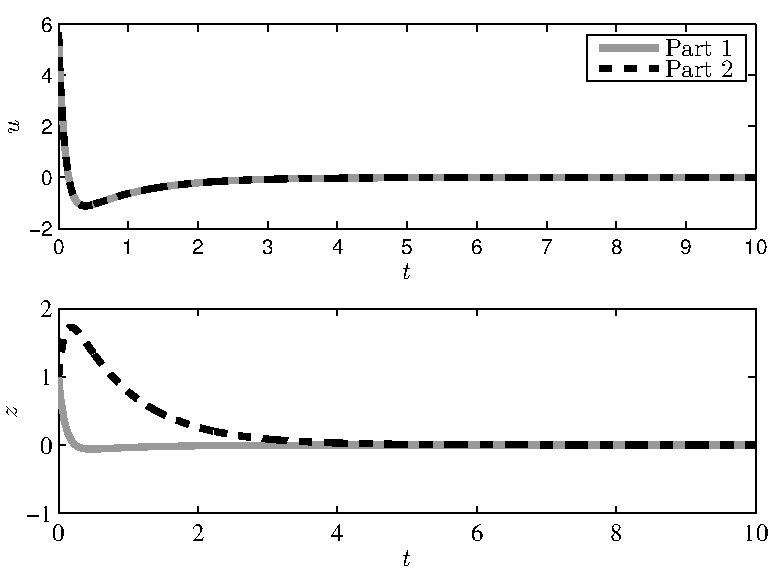
\includegraphics[width=4in]{\figurepath/prob5.pdf}
    \caption{Output and control history plots for the given system, with part 1 and part 2 corresponding to different regulated outputs $z$.\label{fig:prob5}}
  \end{figure}

  From this plot we can see that the system in part 1 has much better performance.
  This is because it has a stable zero at $s=-1$ as opposed to the system in part 2 which has a non-minimum phase zero at $s=1$.

  \clearpage
  \section*{Code}

  \lstinputlisting{\codepath/Problem_1.m}
  \lstinputlisting{\codepath/Problem_2.m}
  \lstinputlisting{\codepath/Problem_5.m}

\end{document}
